\documentclass[12pt]{article}
\usepackage[utf8]{inputenc} % Pacote para acentuação gráfica
%\usepackage[T1]{fontenc}
\usepackage[brazil]{babel} % nomes das estruturas em pt-br
%\usepackage{hyperref}
\usepackage{indentfirst} % indenta primeiro paragráfo após título
\usepackage{setspace} % pacote para alterar espaçamento entre linhas
%\setlength{\parindent}{1cm} % define o tamanho da indentação
%\setlength{\parskip}{0.3cm} % define o espaçamento vertical entre parágrafos
\usepackage[top = 2cm, left = 2cm, bottom = 2cm, right = 2cm]{geometry} % define as margens do documento
\usepackage{fancyhdr} % pacote para numeração de páginas
\usepackage{hyperref}
\usepackage[table,xcdraw]{xcolor} % tabela colorida
\usepackage{float} % força posição de tabelas e figuras
\usepackage{graphicx}

\usepackage{xcolor}
% Definindo novas cores
\definecolor{verde}{rgb}{0.25,0.5,0.35}
\definecolor{jpurple}{rgb}{0.5,0,0.35}
% Configurando layout para mostrar codigos Java
\usepackage{listings}
\lstset{
	language=Java,
	basicstyle=\ttfamily\small,
	keywordstyle=\color{jpurple}\bfseries,
	stringstyle=\color{red},
	commentstyle=\color{verde},
	morecomment=[s][\color{blue}]{/**}{*/},
	extendedchars=true,
	showspaces=false,
	showstringspaces=false,
	numbers=left,
	numberstyle=\tiny,
	breaklines=true,
	backgroundcolor=\color{cyan!10},
	breakautoindent=true,
	captionpos=b,
	xleftmargin=0pt,
	tabsize=4
}
\pagestyle{empty}

\begin{document}
	
\title{\textbf{{\Huge 1Z0-808 - Notas de Estudo}}} % Título
\author{\textbf{{\Large Ricardo Alvarenga}}} % Autor
\date{\textbf{{\Large 2024}}} % Data
\maketitle % Criar
\thispagestyle{empty} % remove número da página
\newpage

\section*{Como Tirar a Certificação Entre 3 e 6 Meses de Estudo}

Referência: \url{https://www.youtube.com/watch?v=t-7GVhoM0bY&t=889s&ab_channel=Jos%C3%A9Castilho-DesenvolvedorDisputado}

\subsection*{Por Quê Tirar a Certificação Java}

\begin{itemize}
	\item Poucos profissionais são certificados;
	\item Gera reconhecimento;
	\item São duas certificações, a primeira \textbf{Java SE Programmer I exam (1Z0-808)}. A segunda querer a primeira e possui várias áreas distintas;
\end{itemize}

\subsection*{Método Sugerido}

\begin{itemize}
	\item Aprender a linguagem, não começar por livro preparatório. Usar livros básicos primeiro;
	\item Estudar com data definida;
	\item "Comer" um livro de certificação;
	\item Usar várias metodologias. Alguns assuntos são assimilados melhor com leitura, outros com vídeos, outros \textit{codando} e vendo funcionar;
	\item Fazer muitos simulados. Simular provas até conseguir notas altas em várias provas simuladas;
	\item Aprender com os erros e acertos dos simulados;
	\item Repetir o ciclo de fazer simulados e analisar erros e acertos, várias vezes;
\end{itemize}

\newpage

\setcounter{page}{1} % reset contador de página
\pagenumbering{Roman}
\tableofcontents % cria sumário
\pagestyle{fancy}
\fancyfoot[C]{\thepage} % Adiciona o número da página no centro do rodapé
\newpage

\listoffigures % lista de figuras
\newpage

\setcounter{page}{1} % reset contador de página
\pagenumbering{arabic}
\pagestyle{fancy}
\fancyfoot[C]{\thepage}


\section{Java Basics}
\subsection{Define the scope of variables}

O escopo é o que determina em que pontos do código uma variável pode ser usada.

\subsubsection{Variáveis locais}

Chamamos de locais as variáveis declaradas dentro de métodos ou construtores. Antes de continuar, vamos estabelecer uma regra básica: o ciclo de vida de uma variável local vai do ponto onde ela foi declarada até o fim do daquele bloco.

Quando uma variável sai do escopo ela não pode mais ser usada e seu valor é perdido. A qualquer momento o JVM pode realocar a memória ocupada por ela.

Mas o que é um bloco? Podemos entender como bloco um trecho de código entre chaves \textbf{\textit{{}}}. Pode ser um método, um construtor, o corpo de um \textbf{\textit{if}}, de um \textbf{\textit{for}} etc.:

\begin{lstlisting}
public void m1() { // inicio do bloco do metodo
	int x = 10; // variavel local do metodo
	
	if (x >= 10) { // inicio do bloco do if
		int y = 50; // variavel local do if
		System.out.print(y);
	} // fim do bloco do if
} // fim do bloco do metodo
\end{lstlisting}

Analisando esse código, temos uma variável \textbf{\textit{x}}, que é declarada no começo do método. Ela pode ser utilizada durante todo o corpo do método. Dentro do \textbf{\textit{if}}, declaramos a variável \textbf{\textit{y}}. \textbf{\textit{y}} só pode ser utilizada dentro do corpo do \textbf{\textit{if}}, delimitado pelas chaves. Se tentarmos usar \textbf{\textit{y}} fora do corpo do \textbf{\textit{if}}, teremos um erro de compilação, pois a variável saiu do seu escopo.

Tome cuidado especial com loops \textbf{\textit{for}}. As variáveis declaradas na área de inicialização do loop só podem ser usadas no corpo do loop:

\begin{lstlisting}
for (int i = 0, j = 0; i < 10; i++)
j++;

System.out.println(j); // erro, ja nao esta mais no escopo
\end{lstlisting}

Parâmetros de métodos também podem ser considerados variáveis locais ao método, ou seja, só podem ser usados dentro do método onde foram declarados:

\begin{lstlisting}
class Teste {
	
	public void m1(String bla) {
		System.out.print(bla);
	}
	
	public void m2() {
		// erro de compilacao pois bla nao existe neste
		// escopo
		System.out.println(bla);
	}
}
\end{lstlisting}

Os parâmetros podem ser primitivos ou objetos. Um método pode ter até 255 parâmetros. Essas variáveis fazem parte do escopo do bloco do método inteiro e são definidas na declaração do método.
\begin{lstlisting}
float findMilesPerHour(float milesTraveled, float hoursTraveled){
	//o metodo contem dois parametros
	return milesTraveled / hoursTraveled;
}
\end{lstlisting}

\subsubsection{Variáveis de instância}

Variáveis de instância ou variáveis de objeto são os atributos dos objetos. São declaradas dentro da classe, mas fora de qualquer método ou construtor. Fazem parte do escopo da classe. Podem ser acessadas por qualquer membro da classe e ficam em escopo enquanto o objeto existir:

\begin{lstlisting}
class Pessoa {
	// variavel de instancia ou variavel de objeto
	String nome;
	
	public void setNome(String n) {
		// acessando a variavel de instancia no metodo
		this.nome = n;
	}
}
\end{lstlisting}

\subsubsection{Variáveis estáticas (class variables)}

Podemos declarar variáveis que são compartilhadas por todas as instâncias de uma classe usando a palavra chave \textbf{\textit{static}}. Essas variáveis estão no escopo da classe, e lá ficarão enquanto a classe estiver carregada na memória (enquanto o programa estiver rodando, na grande maioria dos casos).

\begin{lstlisting}
class Pessoa {
	static int id = 1;
}
	
class Teste {
	public static void main(String[] args) {
		Pessoa p = new Pessoa();
		System.out.println(p.id); // acessando pelo objeto. id = 1
		System.out.println(Pessoa.id); // acessando direto pela classe.
		                               // id = 1
		p.id ++; // soma 1
		System.out.println(Pessoa.id); // id = 2
		p.id ++;
		Pessoa pp = new Pessoa(); 
		p.id ++;
		System.out.println(pp.id); // id = 4
		System.out.println(Pessoa.id); // id = 4
	}
}
\end{lstlisting}

No caso de variáveis \textbf{\textit{static}}, não precisamos ter uma referência para usá-las e podemos acessá-las diretamente a partir da classe, desde que respeitando as regras de visibilidade da variável.

\subsubsection{Variáveis com o mesmo nome}

Logicamente, não é possível declarar duas variáveis no mesmo escopo com o mesmo nome:

\begin{lstlisting}
public void bla() {
	int a = 0;
	int a = 10;// erro
}
\end{lstlisting}

Mas, eventualmente, podemos ter variáveis em escopos diferentes que podem ser declaradas com o mesmo nome. Em casos em que possa haver ambiguidade na hora de declará-las, o próprio compilador irá emitir um erro evitando a confusão.

Por exemplo, não podemos declarar variáveis de classe e de instância com o mesmo nome:

\begin{lstlisting}
class Bla {
	static int a;
	int a; // erro de compilacao,
}
...
System.out.println(new Bla().a); // qual variavel estamos acessando?
\end{lstlisting}

Também não podemos declarar variáveis locais com o mesmo nome de parâmetros:

\begin{lstlisting}
public void metodo(String par) {
	int par = 0; // erro de compilacao
	
	System.out.println(par); // qual?
}
\end{lstlisting}

Apesar de parecer estranho, é permitido declarar variáveis locais ou parâmetros com o mesmo nome de variáveis de instância ou de classe. Essa técnica é chamada de \textit{shadowing}. Nesses casos, é possível resolver a ambiguidade: para variáveis de classe, podemos referenciar pela própria classe; para variáveis de instância, usamos a palavra chave \textbf{\textit{this}}:

\begin{lstlisting}
class Pessoa {
	
	static int x = 0;
	int y = 0;
	
	public static void setX(int x) {
		// Usando a referencia da classe
		Pessoa.x = x;
	}
	
	public void setY(int y) {
		// usando o this
		this.y = y;
	}
}
\end{lstlisting}
\pagebreak
Quando não usamos o \textbf{\textit{this}} ou o nome da classe para usar a variável, o compilador sempre utilizará a variável de menor escopo:

\begin{lstlisting}
class X {
	int a = 10;
	
	public void metodo() {
		int a = 20; // shadowing
		System.out.println(a); // imprime 20
	}
}
\end{lstlisting}

\subsubsection{Difference Between \textit{Life} and \textit{Scope} For Local Variables}

\textbf{\textit{Life:}} A local variable is \textit{alive} as long as its Stack frame is on the Stack. In other words, \textit{until the method completes}.

\textbf{\textit{Scope:}} A local variable is in \textit{scope} only within the method in which the variable was declared. When its own method calls another, the variable is alive, but not in scope until its method resumes. \textbf{You can use a variable only when it is in scope}.


% Please add the following required packages to your document preamble:
% \usepackage[table,xcdraw]{xcolor}
% Beamer presentation requires \usepackage{colortbl} instead of \usepackage[table,xcdraw]{xcolor}
\begin{table}[H]
	\begin{tabular}{|ll|}
		\hline
		\multicolumn{2}{|c|}{\cellcolor[HTML]{34FF34}\textit{\textbf{Cenário e Solução}}}                                        \\ \hline
		\multicolumn{1}{|l|}{Variável mais adequada para um contador em um laço?}                        & Variável local        \\ \hline
		\multicolumn{1}{|l|}{Variável deve ser usada para armazenar informações sobre um objeto?}        & Variável de instância \\ \hline
		\multicolumn{1}{|l|}{Que variável deve ser usada para a passagem de informações para um método?} & Parâmetro de método   \\ \hline
	\end{tabular}
\end{table}

\subsection{Define the structure of a Java class}

Nesta seção, iremos entender a estrutura de um arquivo java, onde inserir as declarações de pacotes e imports e como declarar classes e interfaces.

Para entender a estrutura de uma classe, vamos ver o arquivo \textbf{\textit{Pessoa.java}}:

\begin{lstlisting}
// Declaracao de pacote
package br.com.alvarenga.certificacao;
	
// imports
import java.util.Date;
	
// Declaracao da classe
class Pessoa {
	// conteudo da classe
}
\end{lstlisting}

\subsubsection{Pacotes}

Pacotes servem para separar e organizar as diversas classes que temos em nossos sistemas. Todas as classes pertencem a um pacote, sendo que, caso o pacote não seja explicitamente declarado, a classe fará parte do que chamamos de pacote padrão, ou \textbf{\textit{default package}}. Todas as classes no \textbf{\textit{default package}} se enxergam e podem ser utilizadas entre si. Classes no pacote \textbf{\textit{default}} não podem ser importadas para uso em outros pacotes:

\begin{lstlisting}
// Uma classe no pacote padrao
class Pessoa {
	//...
}
\end{lstlisting}

Para definir qual o pacote a que a classe pertence, usamos a palavra-chave \textbf{\textit{package}}, seguida do nome do pacote. Só pode existir um único \textbf{\textit{package}} definido por arquivo, e ele deve ser a primeira instrução do arquivo. Após a definição do \textbf{\textit{package}}, devemos finalizar a instrução com um \textbf{\textit{;}}. Podem existir comentários antes da definição de um pacote:

\begin{lstlisting}
// declaracao do pacote
package br.com.alvarenga.certificacao;
	
class Pessoa {
	//...
}
\end{lstlisting}

\textbf{\textit{Package}} deve ser a primeira instrução de código que temos declarada em nosso arquivo. Comentários não são considerados parte do código, portanto, podem existir em qualquer lugar do arquivo java sem restrições.

Formas para inserir comentários:

\begin{lstlisting}
// comentario de linha

/*
comentario de
multiplas linhas
*/
class /* comentario no meio da linha */ Pessoa {
	
	/**
	*  JavaDoc, repare que a primeira linha do comentario tem
	*  2 asteriscos
	*/
	public void metodo() {
	}
}
\end{lstlisting}

\subsubsection{Classe}

Uma classe é a forma no Java onde definimos os atributos e comportamentos de um objeto. A declaração de uma classe pode ser bem simples, apenas a palavra \textbf{\textit{class}} seguida do nome e de \textbf{\textit{{}}}:

\begin{lstlisting}
class Pessoa {}
\end{lstlisting}

Existem outros modificadores que podem ser usados na definição de uma classe, mas veremos essas outras opções mais à frente, onde discutiremos esses modificadores com mais detalhes.

Vale lembrar que java é case \textit{sensitive} e \textbf{\textit{Class}} é o nome de uma classe e não podemos usá-lo para definir uma nova classe.

Dentro de uma classe, podemos ter variáveis, métodos e construtores. Essas estruturas são chamadas de \underline{\textbf{membros da classe}}.:

\begin{lstlisting}
class Pessoa {
	
	String nome;
	String sobrenome;
	
	Pessoa(String nome, String sobrenome) {
		this.nome = nome;
		this.sobrenome = sobrenome;
	}
	
	public String getNomeCompleto() {
		return this.nome + this.sobrenome;
	}
}	
\end{lstlisting}

% TODO: \usepackage{graphicx} required
\begin{figure}[H]
	\centering
	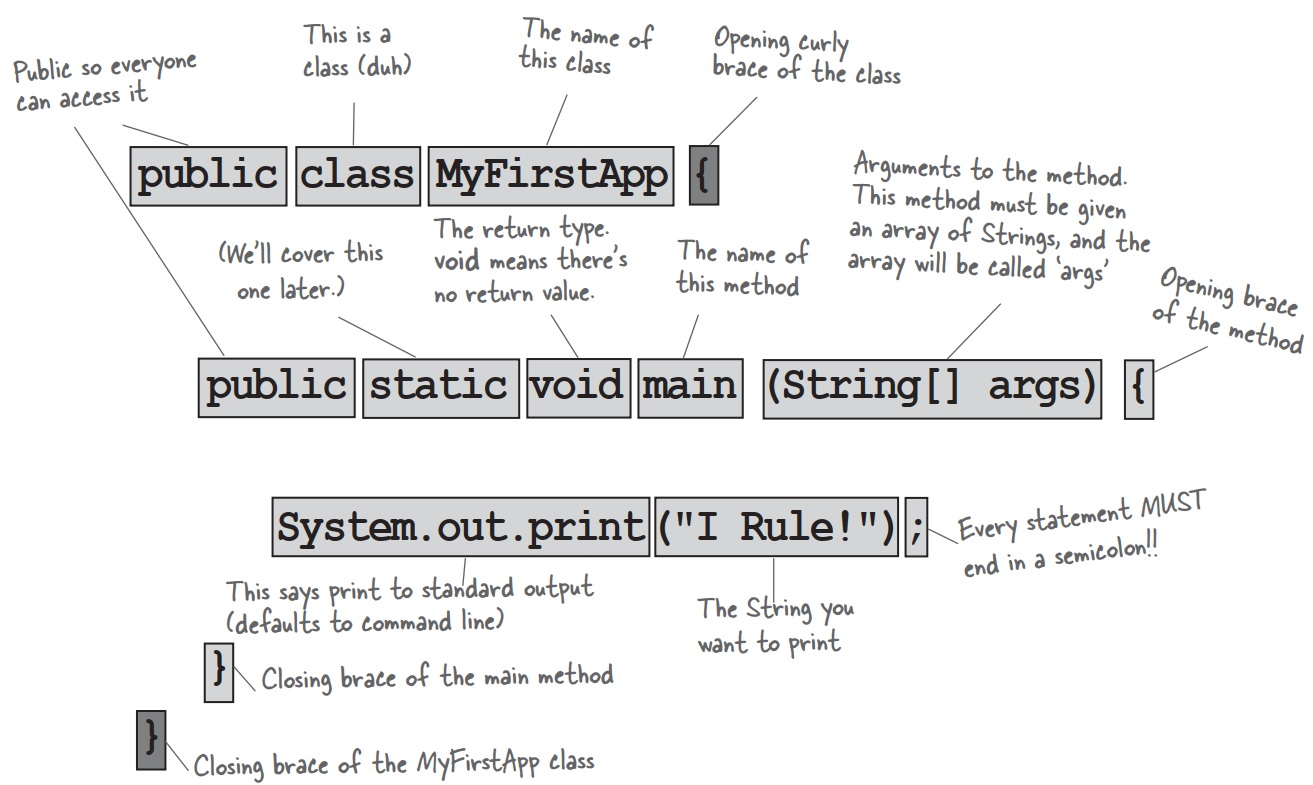
\includegraphics[width=1\linewidth]{figuras/class}
	\caption[Anatomy of a class]{Anatomy of a class}
	\label{fig:class}
\end{figure}

In Java, everything goes in a class. You’ll type your source code file (with a \textit{.java} extension), then compile it into a new class file (with a \textit{.class} extension). When you run your program, you’re really running a class.


\subsubsection{Variáveis}

Usando como exemplo a classe Pessoa definida anteriormente, nome e sobrenome são variáveis. A declaração de variáveis é bem simples, sempre o tipo seguido do nome da variável.

Dizemos que essas são variáveis de instância, pois existe uma cópia delas para cada objeto Pessoa criado em nosso programa. Cada cópia guarda o estado de uma certa instância desses objetos.

Existem ainda variáveis que não guardam valores ou referências para uma determinada instância, mas sim um valor compartilhado por todas as instâncias de objetos. Essas são variáveis estáticas, definidas com a palavra-chave \textbf{\textit{static}}. Veremos mais sobre esse tipo de membro mais à frente.

\subsubsection{Métodos}

A declaração de métodos é um pouquinho diferente pois precisamos do tipo do retorno, seguido do nome do método e seguido de parênteses, sendo que pode ou não haver parâmetros de entrada desse método. Cada parâmetro é uma declaração de variável em si. Essa linha do método, onde está definido o retorno, o nome e os parâmetros é onde temos a assinatura do método. Cuidado, pois a assinatura de um método inclui somente o nome do método e os tipos dos parâmetros.

Assim como variáveis, métodos também podem ser \textbf{\textit{static}}, como veremos mais adiante.

\subsubsection{Construtores}

Uma classe pode possuir zero ou vários construtores. Nossa classe Pessoa possui um construtor que recebe como parâmetros o nome e o sobrenome da pessoa. A principal diferença entre a declaração de um método e um construtor é que um construtor não tem retorno e possui o mesmo nome da classe.

\subsubsection{Métodos com o mesmo nome da classe}

Note que um construtor pode ter um \textbf{\textit{return}} vazio:

\begin{lstlisting}
class X {
	int j = -100;
	
	X(int i) {
		if (i > 1)
		return;
		j = i;
	}
}
\end{lstlisting}

Caso o valor seja maior que \textbf{\textit{1}}, o valor de \textbf{\textit{j}} será \textbf{\textit{-100}}, caso contrário, será o mesmo valor de \textbf{\textit{i}}.

\subsubsection{Interfaces}

Além de classes, também podemos declarar \textit{interfaces} em nossos arquivos java. Para definir uma interface usamos a palavra reservada \textbf{\textit{interface}}:

\begin{lstlisting}
interface Autenticavel {
	
	final int TAMANHO_SENHA = 8;
	
	void autentica(String login, String senha);
}
\end{lstlisting}

Em uma interface, devemos apenas definir a assinatura do método, sem a sua implementação. Além da assinatura de métodos, também é possível declarar constantes em interfaces.

\subsubsection{Múltiplas estruturas em um arquivo}

Em java, é possível definir mais de uma classe/interface em um mesmo arquivo java, embora devamos seguir algumas regras:

\begin{enumerate}
	\item Podem ser definidos em qualquer ordem;
	\item Se existir alguma classe/interface pública, o nome do arquivo deve ser o mesmo dessa classe/interface;
	\item Só pode existir uma classe/interface pública por arquivo;
	\item Se não houver nenhuma classe/interface pública, o arquivo pode ter qualquer nome.
\end{enumerate}

Logo, são válidos:

\begin{lstlisting}
// arquivo1.java
interface Bar {}

class Foo {}
\end{lstlisting}


\begin{lstlisting}
// Foo.java
public class Foo {}

interface X {}
\end{lstlisting}

\subsubsection{Pacotes e imports em arquivos com múltiplas estruturas}

As regras de pacotes e \textbf{\textit{imports}} valem também para arquivos com múltiplas estruturas definidas. Caso exista a definição de um pacote, ela vale para todas as classes/interfaces definidas nesse arquivo, e o mesmo vale para \textbf{\textit{imports}}.

\subsection*{Create executable Java applications with a main method; run a Java program from the command line; produce console output}





\newpage

\subsection*{Import other Java packages to make them accessible in your code}
\subsection*{Compare and contrast the features and components of Java such as: platform independence, object orientation, encapsulation, etc.}

	
\end{document}